

\lstset{language=myasm}

\section{definitive sources}
\begin{frame}{x86-64 assembly}
\begin{itemize}
\item history: AMD constructed 64-bit extension to x86 first
    \begin{itemize}
    \item marketing term: AMD64
    \end{itemize}
\item Intel first tried a new ISA (Itanium), which failed
\item Then Intel copied AMD64
    \begin{itemize}
    \item marketing term: EM64T
        \begin{itemize}\item Extended Memory 64 Technology\end{itemize}
    \item later marketing term: Intel 64
    \end{itemize}
\item both Intel and AMD have manuals --- definitive reference
\end{itemize}
\end{frame}

\begin{frame}
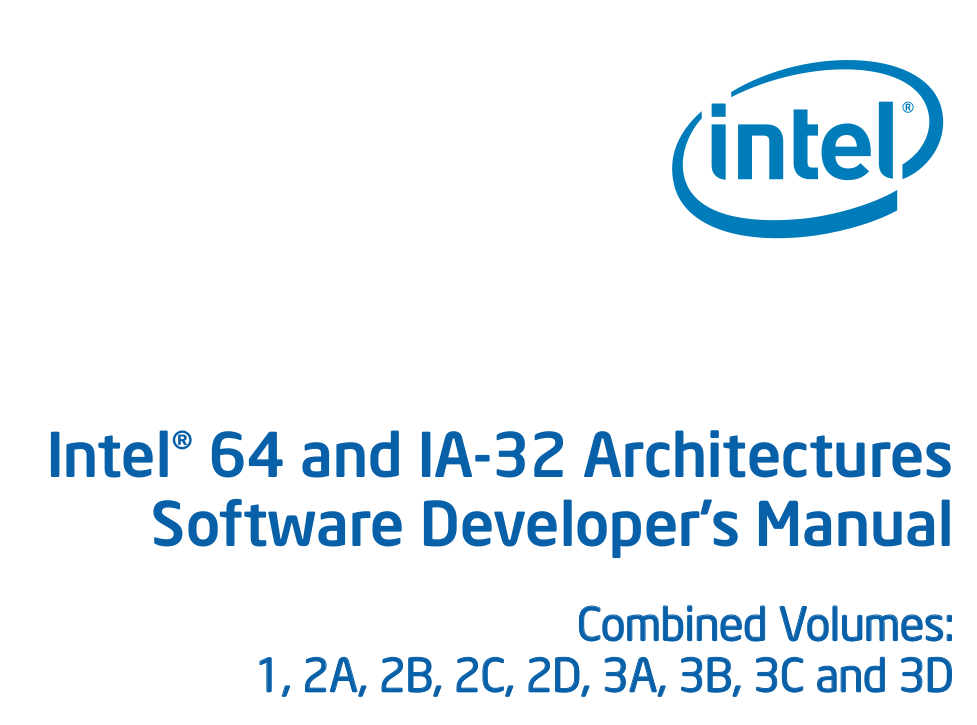
\includegraphics[height=0.9\textheight]{../asm/manual-screenshot}
\end{frame}

\begin{frame}{x86-64 manuals}
\begin{itemize}
\item Intel manuals:
    \begin{itemize}
    \item \small \url{https://software.intel.com/en-us/articles/intel-sdm}
    \item 24 MB, 4684 pages
    \item Volume 2: instruction set reference (2190 pages)
    \end{itemize}
\item AMD manuals:
    \begin{itemize}
    \item \small \url{https://support.amd.com/en-us/search/tech-docs}
    \item ``AMD64 Architecture Programmer's Manual''
    \end{itemize}
\end{itemize}
\end{frame}

\begin{frame}{example manual page}
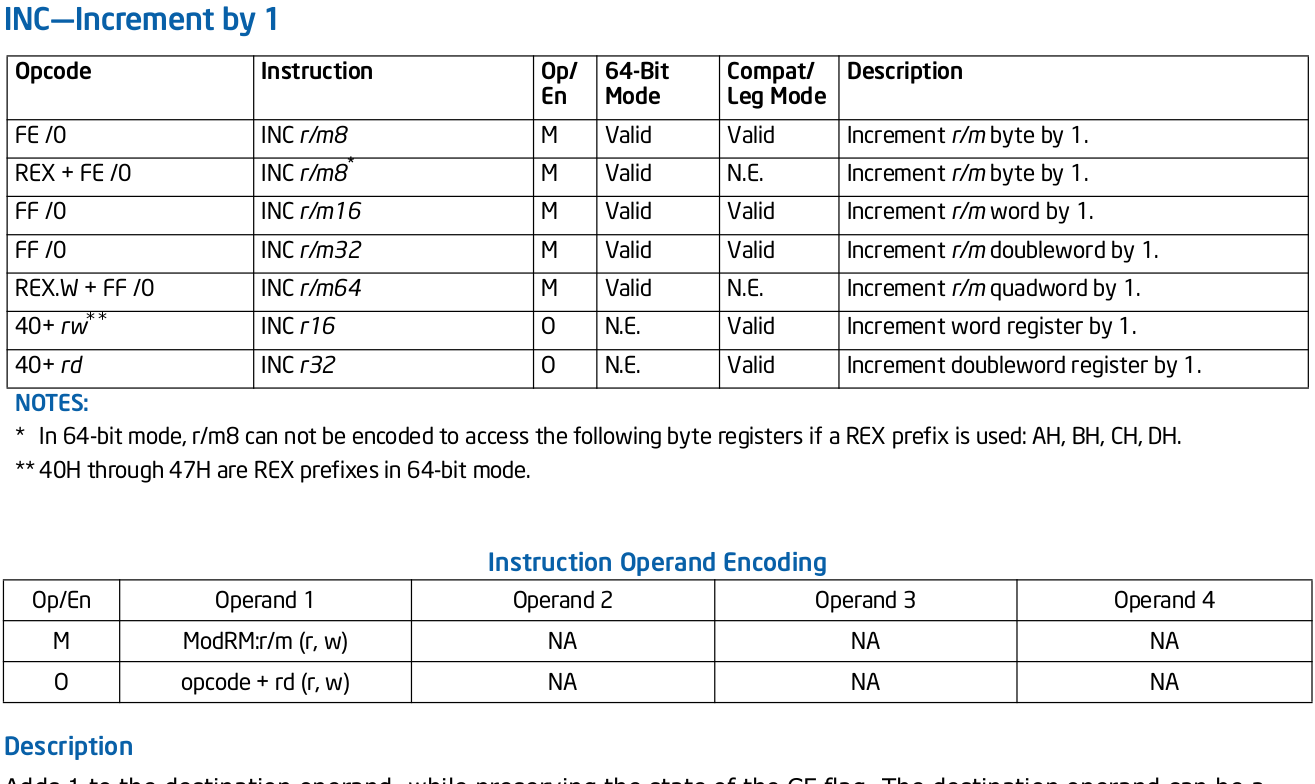
\includegraphics[width=\textwidth]{../asm/example-manual}
\end{frame}

\begin{frame}{instruction listing parts (1)}
    \begin{itemize}
    \item opcode --- first part of instruction encoding
        \begin{itemize}
        \item yes, variable length
        \item ``REX''???
        \item more later (today or next week)
        \end{itemize}
    \item instruction --- Intel assembly skeleton
    \item {\tt r/m32} --- 32-bit memory or register value
    \item 64-bit mode --- does instruction exist in 64-bit mode?
    \item compat/leg mode --- in 16-bit/32-bit modes?
    \end{itemize}
\end{frame}

\begin{frame}{instruction listing parts (2)}
    \begin{itemize}
    \item dscription + operation (later on page)
        \begin{itemize}
        \item text and pseudocode description
        \end{itemize}
    \item flags affected
        \begin{itemize}
        \item flags --- used by {\tt jne}, etc.
        \end{itemize}
    \item exceptions --- how can OS be called from this?
        \begin{itemize}
        \item example: can invalid memory access happen?
        \end{itemize}
    \end{itemize}
\end{frame}
